\documentclass[manuscript,screen,review]{jair}

\usepackage{amsmath}
\usepackage{booktabs}
\usepackage{graphicx}
\usepackage{xcolor}

\newcommand{\modelmetrics}[2]{\textit{Model(s):} #1. \textit{Metrics:} #2.}

% Regular JAIR article submitted for review (not a special track).
% The Associate Editor and publication metadata are assigned by JAIR.
\JAIRTrack{}
\JAIRAE{}
\acmDOI{}
\settopmatter{printacmref=false}

\begin{document}

\title{Guiding Mixture-of-Experts Reasoning via Routing Intervention}

\maketitle

\section{Introduction}

\section{Background}

\section{Related Work}

\section{Routing Intervention}

\section{Experimental Setup}

\paragraph{Current experimental scope.}
All results available at the time of writing use
\texttt{allenai/OLMoE-1B-7B-0924-Instruct} (16 MoE layers, 64 experts,
top-$k=8$).  The current successful runs are GSM8K (1,319 generated traces),
GSM8K with a self-check prompt (1,319), MATH (1,500), MATH with a self-check
prompt (1,500), and ProcessBench (400 given-solution traces).  All five have
complete router and hidden-state tensors and outputs for Experiments 1--5.
The current PRM800K launch is not a completed experiment: its Experiment~1
JSONL is empty, and downstream stages produced zero-input placeholder files.
Older, corrected-label PRM800K event and full-trace probe outputs over 10,833
traces are retained as explicitly marked legacy evidence.  Unless stated
otherwise, event windows contain five tokens on each side of the event.
In addition, Experiment~0a is an auxiliary judge-validation study: completed
static-reward baselines and a completed same-model LLM-as-a-judge final fit
optimize a Qwen3.6-27B prompt for sentence-level Schoenfeld episode
classification.  This judge experiment evaluates annotation capability and is
not evidence about Qwen router dynamics.  Experiment~0b is
a separate representation-probe replication: it teacher-forces the 38
released DeepSeek-R1 Schoenfeld traces through the official GPTQ 4-bit
\texttt{Qwen/Qwen3.5-35B-A3B-GPTQ-Int4} checkpoint and asks whether the label
of the next sentence is linearly decodable at its causal pre-sentence
boundary.  It is an auxiliary hidden-state experiment rather than a routing
result from the OLMoE pipeline.

\paragraph{Implemented analysis pipeline.}
The repository implements trace generation or ingestion (Experiment 1),
token-level router and optional hidden-state extraction (Experiment 2),
event-centered routing with matched within-trace controls, geometry--routing
correlation (Experiment 3), prospective prefix probes (Experiment 4), and
expert phase/co-activation/transition analysis (Experiment 5).  Offline tools
also support high-precision relabelling, rebuilding multi-dataset taxonomy
summaries, full-trace layerwise linear probes over router, hidden, or combined
features, and a trace-length/structure baseline.  The full pipeline runs
Experiments 1--5 and extracts hidden states by default; the latter and
Experiment 4 can be disabled together when storage is constrained.
Experiment~0a is run separately: a local \texttt{llama.cpp} server supplies
Qwen3.6-27B predictions while GEPA optimizes the instruction.  The current
version supplies the problem statement and previous/current/next response
units, uses 21 audited synthetic contrastive demonstrations, supports
an informative same-model LLM-as-a-judge reward alongside the earlier static
rewards, and evaluates prompt-selection rules with nested response-grouped
cross-validation.

Experiment~0b separately aligns the released sentence annotations to their
original responses, extracts one 2,048-dimensional boundary vector at each of
41 hidden-state indices, trains layerwise episode probes, and applies their
selected layers to reference or supplied solutions from four external math
benchmarks.  Only the boundary vectors are stored; Qwen does not regenerate
the released or benchmark solutions.

The separate correlation pipeline now has one completed benchmark-scale run:
500 single-sample MATH-500 generations from Qwen3.5-35B-A3B, replayed through
the matching checkpoint with router and hidden-state features.  Results from
this run are reported separately because they use a different model and
protocol from the five OLMoE conditions above.  The remaining correlation
benchmarks and repeated-attempt evaluations are still pending.

\paragraph{Table model and metric conventions.}
Every table caption identifies the evaluated model or models and the metrics
shown.  For classification, accuracy is the fraction of exact label matches,
balanced accuracy is the unweighted mean of class recalls, precision and
recall have their standard true-positive definitions, macro-F1 is the
unweighted mean of per-class F1, and AUROC measures score ranking across the
positive and negative classes.  Cohen's $\kappa$ is chance-corrected nominal
agreement, Kendall's $\tau_b$ is rank agreement under the fixed episode-label
ordering, and the Experiment~0a composite averages their equal-weight
$[0,1]$ rescalings.  Routing entropy is Shannon entropy of the softmax router
distribution; switch rate is the fraction of top-$k$ experts replaced from
the preceding token; top-$k$ overlap is adjacent-token Jaccard overlap; and
router margin is the top-1 minus top-2 router probability.  Unless a caption
states otherwise, $N$ and support are observation counts, $r$ is a Pearson-
family correlation coefficient, and confidence intervals are percentile
bootstrap intervals.

\paragraph{Prospective probe design and status.}
Experiment 4 pools only the first 25\%, 50\%, or 75\% of each trace and trains
separate trace-grouped logistic probes from structure-only, router-only,
hidden-only, and combined hidden/router features.  It evaluates final
incorrectness and whether a gold first error remains beyond the observed
prefix, excluding traces whose error has already occurred for the latter
target.  Outputs include out-of-fold AUROC, balanced accuracy, F1, and
trace-bootstrap confidence intervals.  This pipeline is implemented and
has completed for all five current conditions.  Final-incorrectness probes are
available everywhere.  Future-first-error probes are available only for
ProcessBench because the generated datasets do not have gold error-step
annotations.

\paragraph{Schoenfeld boundary-probe design.}
Experiment~0b starts from 3,125 annotated units in 38 released DeepSeek-R1 SAT
responses.  It excludes the 38 synthetic \texttt{</think>} closing units,
which are all labelled Monitor, leaving the paper-matched 3,087 units.  Qwen
receives each SAT instruction as the user message and the released response as
a teacher-forced assistant continuation.  For a target unit, the feature is
the hidden state immediately before its first token, so the probe sees the
problem and preceding response but cannot read the target sentence.  Hidden-
state index 0 is the embedding output and indices 1--40 are the successive
language-model layers.

At each index, seven separate target-versus-rest logistic regressions use raw
activations, balanced class weights, L2 regularization with $C=1$, and no
standardization or PCA.  The paper-matched protocol uses a target-stratified
80/20 sentence split with seed 42.  This is a replication choice rather than
a strong generalization design: all 38 response IDs occur in both partitions.
The reported layer for each target maximizes accuracy on that same test split.
For qualitative transfer inspection, the selected probes are then applied to
20 examples each from GSM8K, MATH, PRM800K, and ProcessBench.  The seven binary
scores are independently trained and uncalibrated; their argmax is an
inspection label, not a multiclass probability or new gold annotation.

\paragraph{Important provenance note.}
The event-label heuristic was made substantially more conservative after the
first experimental run.  Taxonomy, event-routing, and expert-event outputs
for the five current conditions were regenerated with the corrected labels,
and their JSONL files pass line-by-line JSON validation.  The separate
PRM800K relabelled files and full-trace probe outputs predate the current
pipeline run and are never pooled with current estimates.  SLURM's printed
``Pipeline complete'' banner is not treated as evidence of success: both
PRM800K logs contain explicit zero-input errors even though the shell script
continued to that banner.  Historical logs also include a CUDA out-of-memory
failure and several OLMoE/Qwen MoE-generation logs that end mid-progress; no
Qwen routing-result artifacts are present, so these are excluded rather than
counted as robustness runs.  The separate Qwen judge artifacts from
Experiment~0a and the Qwen3.5 boundary-probe artifacts from Experiment~0b are
complete.  Repeated cgroup swap-limit warnings also appear in the successful
jobs and are treated as environmental warnings, not failures.

\section{Results}

\subsection{GEPA-optimized episode judge}

Experiment~0a evaluates whether prompt optimization improves a local judge for
the seven adapted Schoenfeld episode labels: Read, Analyze, Plan, Implement,
Explore, Verify, and Monitor.  The model was the Q4\_K\_XL quantization of
Qwen3.6-27B served by \texttt{llama.cpp} on one RTX 3090.  All splits preserve
complete responses, preventing neighboring units from crossing partitions.

\paragraph{Preliminary single-split runs.}
With seed 42, the 38 responses were divided into 26 training, 6 validation,
and 6 test documents (2,382/407/336 units).  These first runs classified the
current unit without neighboring context and optimized per-unit exact match.

\begin{table}[t]
\centering
\caption{Preliminary Experiment~0a judge agreement.  The composite rescales Cohen's
$\kappa$ and Kendall's $\tau_b$ from $[-1,1]$ to $[0,1]$ and averages them.
Coverage was 100\% in every row.  \modelmetrics{Qwen3.6-27B
\texttt{Q4\_K\_XL}, used as the episode-label judge}{exact-match accuracy,
Cohen's $\kappa$, Kendall's $\tau_b$, their rescaled composite, and valid-output
coverage}}
\label{tab:exp0a-judge}
\begin{tabular}{lrrrr}
\toprule
Evaluation & Accuracy & $\kappa$ & $\tau_b$ & Composite \\
\midrule
Seed validation      & 0.6388 & 0.5581 & 0.4810 & 0.7598 \\
Optimized validation & 0.6855 & 0.6074 & 0.5847 & 0.7980 \\
Optimized test       & 0.6607 & 0.5710 & 0.6066 & 0.7944 \\
Few-shot validation  & 0.6806 & 0.6078 & 0.5830 & 0.7977 \\
Few-shot test        & \textbf{0.6994} & \textbf{0.6178} &
\textbf{0.6667} & \textbf{0.8211} \\
\bottomrule
\end{tabular}
\end{table}

The matched few-shot run used the same seed, document split, model, and GEPA
budget, adding seven gold training examples to the instruction.  It performs
better than the optimized base condition on the held-out test set: accuracy
rises from 66.07\% to 69.94\% (+3.87 percentage points), Cohen's $\kappa$ from
0.5710 to 0.6178, Kendall's $\tau_b$ from 0.6066 to 0.6667, and composite
agreement from 0.7944 to 0.8211.  GEPA itself does not improve the few-shot
validation result: the seed and selected optimized prompts both score 68.06\%
accuracy.  The current comparison therefore favors few-shot prompting for
held-out generalization, whereas the measurable GEPA optimization gain is
confined to the base-prompt condition.

\paragraph{Context-aware nested cross-validation.}
The revised protocol excludes the same six responses from model selection and
runs five outer folds over the remaining 32 responses.  Within each fold,
five responses form the inner validation set and all others outside the outer
fold form the GEPA training set.  Each request includes the problem statement,
previous unit, current unit, and next unit.  The seed instruction includes 21
audited synthetic contrastive demonstrations.  GEPA receives inverse-frequency
weighted exact match, whose split mean is balanced accuracy; the safety
selector compares either balanced accuracy or macro-F1 and rejects any
candidate whose class recall falls by more than the configured threshold.

\paragraph{Informative same-model reward.}
The current implementation can replace the static GEPA reward with an
LLM-as-a-judge call to the same Qwen3.6-27B model.  For each candidate label,
the judge returns a short free-text explanation plus four diagnostic scores
from 1 to 5: gold agreement, functional fit, contextual coherence, and boundary
precision.  Their normalized weighted mean is used only as GEPA's optimization
signal, with respective weights 0.40, 0.25, 0.15, and 0.20.  Gold-label
accuracy, balanced accuracy, macro-F1, and per-class recall remain the
independent selection and reporting criteria.  The judge runs deterministically
with model reasoning disabled.  Every judge call is persisted as JSONL with
its component scores, normalized score, and free-text explanation, permitting
a direct audit of feedback quality.  Tables~\ref{tab:exp0a-cv} and
\ref{tab:exp0a-classes} remain static-reward cross-validation baselines; the
completed LLM-judge final fit is reported separately below because its reused
validation set is a prompt-development set rather than an outer-fold estimate.

\begin{table}[t]
\centering
\caption{Aggregate selected-prompt outer-fold results over 2,789 units.
``Balanced light'' is the earlier 0.10 recall-gate run; the macro-F1 runs use a
0.05 gate.  The six excluded responses were not evaluated.
\modelmetrics{Qwen3.6-27B \texttt{Q4\_K\_XL}, used as the episode-label
judge}{exact-match accuracy, balanced accuracy, macro-F1, and the rescaled
$\kappa$/$\tau_b$ composite}}
\label{tab:exp0a-cv}
\begin{tabular}{lrrrr}
\toprule
Selection / budget & Accuracy & Balanced acc. & Macro-F1 & Composite \\
\midrule
Balanced / light & 0.6701 & 0.6753 & 0.6480 & 0.8031 \\
Macro-F1 / light & \textbf{0.6734} & \textbf{0.6796} &
\textbf{0.6505} & \textbf{0.8063} \\
Macro-F1 / heavy & 0.6669 & 0.6737 & 0.6437 & 0.8030 \\
\bottomrule
\end{tabular}
\end{table}

Macro-F1 selection with the light budget is the strongest cross-validated
configuration, but its advantage over balanced-accuracy selection is small:
+0.32 accuracy points, +0.43 balanced-accuracy points, and +0.24 macro-F1
points.  At the response level it wins on 15 documents, loses on 13, and ties
on 4, so the observed gain is not stable across documents.  The light run
selects a GEPA-optimized prompt in three of five folds; the recall gate retains
the seed prompt in the other two because Plan or Monitor recall falls too far.

Increasing the budget does not help.  The heavy run selects an optimized
prompt in only two folds and is 0.65 accuracy points and 0.68 macro-F1 points
below the light run.  Paired predictions show 38 units correct only under
light versus 20 correct only under heavy.  This difference is concentrated in
fold 5, where light discovers and selects a strong candidate whereas heavy
retains the seed after its candidate violates the Analyze recall gate.
Independent heavy search is therefore not a superset of light search and can
discard a better prompt found by a smaller run.

\begin{table}[t]
\centering
\caption{Per-class outer-fold performance for the best current configuration,
macro-F1 selection with the light GEPA budget.  \modelmetrics{Qwen3.6-27B
\texttt{Q4\_K\_XL}, used as the episode-label judge}{class support, precision,
recall, and F1}}
\label{tab:exp0a-classes}
\begin{tabular}{lrrrr}
\toprule
Class & Support & Precision & Recall & F1 \\
\midrule
Read      & 318 & 0.798 & 0.770 & 0.784 \\
Analyze   & 685 & 0.757 & 0.632 & 0.689 \\
Plan      & 205 & 0.524 & 0.590 & 0.555 \\
Implement & 650 & 0.880 & 0.722 & 0.793 \\
Explore   & 193 & 0.679 & 0.492 & 0.571 \\
Verify    & 538 & 0.669 & 0.606 & 0.636 \\
Monitor   & 200 & 0.364 & 0.945 & 0.526 \\
\bottomrule
\end{tabular}
\end{table}

The revised objective improves overall balance only marginally and does not
resolve Monitor overprediction.  The model emits Monitor 519 times for 200
gold Monitor units; the leading errors are Verify$\rightarrow$Monitor (127),
Plan$\rightarrow$Monitor (65), and Explore$\rightarrow$Monitor (42).  The
annotation audit flags 180/3,125 units (5.76\%), including 145 multiline units
and 49 structural/control markers such as \texttt{</think>} and ``Final
Answer.''  These artifacts plausibly inflate Monitor recall while depressing
precision and should be reviewed before further optimization.

All runs retain 100\% final-output coverage and complete without OOM failures,
but the light and heavy jobs log 31 and 28 truncated LM responses during
optimization.  Moreover, the outer folds currently evaluate only the
safety-selected prompt, not both seed and optimized prompts, so they do not
directly estimate GEPA's paired outer-fold gain.  Finally, the six responses
excluded from current CV were inspected in the preliminary experiments; they
are locked from the current code path but no longer constitute a pristine
research holdout.  The judge should therefore not replace validated annotation
until structural artifacts are adjudicated, decoding is constrained, paired
outer evaluation is added, and a genuinely unseen external test set is
designated.

\paragraph{Completed LLM-judge final fit.}
The August 11, 2026 run uses seed 42, the 21-example context-aware few-shot
prompt, and the same-model informative reward on the original response-grouped
26/6/6 split (2,382/407/336 units).  Seed and optimized prompts both return a
valid label for all 407 validation units.  Table~\ref{tab:exp0a-llmjudge}
reports exact gold-label metrics rather than the LLM judge's diagnostic score.

\begin{table*}[t]
\centering
\caption{Context-aware LLM-judge final-fit results on the 407-unit
prompt-development validation set.  Coverage is 100\% in both rows.  The locked test
is not evaluated.  \modelmetrics{Qwen3.6-27B \texttt{Q4\_K\_XL}, used both
for episode-label prediction and the same-model GEPA reward}{exact-match
accuracy, balanced accuracy, macro-F1, Cohen's $\kappa$, Kendall's $\tau_b$,
absolute change, and valid-output coverage}}
\label{tab:exp0a-llmjudge}
\begin{tabular}{lrrrrr}
\toprule
Prompt & Accuracy & Balanced acc. & Macro-F1 & $\kappa$ & $\tau_b$ \\
\midrule
21-example seed & 0.6683 & 0.6765 & 0.6132 & 0.5988 & 0.5904 \\
GEPA optimized  & \textbf{0.7543} & \textbf{0.7769} & \textbf{0.7270} &
\textbf{0.6968} & \textbf{0.6832} \\
\midrule
Absolute change & +0.0860 & +0.1003 & +0.1138 & +0.0980 & +0.0929 \\
\bottomrule
\end{tabular}
\end{table*}

The optimized prompt fixes 49 seed errors and regresses on 14 previously
correct units, a net gain of 35.  All six validation responses improve, with
response-level accuracy gains from 2.0 to 13.8 percentage points.  Its primary
effect is to curb the seed prompt's overuse of Monitor: Monitor predictions
fall from 74 to 43, including nine corrections from Monitor to true Plan and
15 from Monitor to true Verify.  Recall rises most for Plan (+28.13 points),
Explore (+23.53), Verify (+14.29), and Analyze (+8.20).  Monitor recall falls
slightly from 1.000 to 0.944, but precision rises from 0.243 to 0.395.  The
selected prompt still has weak Monitor precision and Analyze recall, and the
remaining errors concentrate at the Analyze/Implement/Verify boundaries and
Verify$\rightarrow$Monitor.  Implement is the only class whose F1 decreases,
from 0.839 to 0.825, because its additional predictions include more false
positives.

\begin{table}[t]
\centering
\caption{Per-class recall and optimized F1 for the completed LLM-judge final
fit.  \modelmetrics{Qwen3.6-27B \texttt{Q4\_K\_XL}, used both for
episode-label prediction and the same-model GEPA reward}{class support, seed
and optimized recall, and optimized per-class F1}}
\label{tab:exp0a-llmjudge-classes}
\begin{tabular}{lrrrr}
\toprule
Class & Support & Seed recall & Opt. recall & Opt. F1 \\
\midrule
Read      &  45 & 0.778 & 0.756 & 0.791 \\
Analyze   & 122 & 0.598 & 0.680 & 0.744 \\
Plan      &  32 & 0.531 & 0.813 & 0.722 \\
Implement & 103 & 0.786 & 0.825 & 0.825 \\
Explore   &  17 & 0.471 & 0.706 & 0.686 \\
Verify    &  70 & 0.571 & 0.714 & 0.763 \\
Monitor   &  18 & 1.000 & 0.944 & 0.557 \\
\bottomrule
\end{tabular}
\end{table}

The internal same-model reward rises from 0.7264 for the seed to 0.8196 for
the selected candidate.  The optimization trace contains 145 candidates, 144
full validation evaluations, and 60,767 persisted judge calls, of which 148
are judge-output errors.  A text audit finds 37 validation units for which the
judge explicitly disputes the corpus gold label in at least one evaluation,
showing that the reward itself detects annotation-sensitive boundaries rather
than consistently treating gold as semantically authoritative.  The structural
audit flags 29 validation units; their accuracy remains 72.4\% under both
prompts, so the gain comes entirely from otherwise unflagged units.

GEPA expands the instruction from 21 to 40 demonstrations and from 7,648 to
32,717 characters.  The extra rules and examples target observed corpus edge
cases, raising inference cost and the risk of learning annotation conventions
rather than a portable episode taxonomy.  More importantly, GEPA evaluates
145 candidates against the same six-response validation set used for final
selection.  The nominal 407 units are also correlated within responses, and
only one optimization seed is available.  The result files explicitly record
\texttt{locked\_test\_evaluated: false} and \texttt{test: null}.  The observed
gain is therefore strong evidence of successful prompt optimization on the
development distribution, but not a held-out generalization estimate.  The
prompt should be frozen and compressed or ablated before a one-time test on
genuinely unseen responses.

\subsection{Schoenfeld episode-boundary probes}

Experiment~0b tests a different annotation mechanism from the generative
judge in Experiment~0a.  It asks whether Qwen's representation of the prefix
immediately before a sentence contains linearly accessible information about
the upcoming Schoenfeld episode.  It therefore measures prospective
prefix-state decodability, not semantic classification after reading the
sentence and not the latent dynamics of a Qwen-generated trace.

\paragraph{Within-corpus results.}
Table~\ref{tab:schoenfeld-boundary-probes} reports the accuracy-selected layer
for each one-versus-rest target.  AUROC is 0.835--0.934 and balanced accuracy
is 0.740--0.862, demonstrating substantial within-split ranking signal.
Implement is strongest at the natural threshold (F1 0.771), followed by
Verify (0.726) and Read (0.704).  Analyze is intermediate.  Plan, Explore, and
Monitor have F1 below 0.50.  Their nominal accuracies are also 0.96--1.06
percentage points below an always-negative majority classifier, so accuracy
alone gives a misleading impression for these rare targets.

\begin{table*}[t]
\centering
\caption{Accuracy-selected Schoenfeld boundary probes on the sentence-level
test split.  Prevalence is over all 3,087 units.  $\Delta$Maj. subtracts the
always-negative accuracy.  Balanced accuracy is derived from the saved test
confusion matrix.  Layer selection and evaluation use the same test split and
are therefore selection-optimistic.  \modelmetrics{
\texttt{Qwen/Qwen3.5-35B-A3B-GPTQ-Int4} as a frozen hidden-state encoder, with
one-versus-rest logistic probes}{target prevalence, selected hidden-state
layer, accuracy, accuracy minus the majority baseline, balanced accuracy, F1,
and AUROC}}
\label{tab:schoenfeld-boundary-probes}
\resizebox{\textwidth}{!}{%
\begin{tabular}{lrrrrrrr}
\toprule
Target & Prevalence & Layer & Accuracy & $\Delta$Maj. & Balanced acc. & F1 & AUROC \\
\midrule
Read      & 12.21\% & 34 & 0.9239 & +0.0461 & 0.8476 & 0.7044 & 0.9338 \\
Analyze   & 25.62\% & 36 & 0.8107 & +0.0669 & 0.7669 & 0.6465 & 0.8348 \\
Plan      &  7.29\% & 39 & 0.9175 & -0.0096 & 0.7405 & 0.4848 & 0.8551 \\
Implement & 21.87\% & 38 & 0.8964 & +0.1151 & 0.8617 & 0.7714 & 0.9305 \\
Explore   &  6.74\% & 40 & 0.9223 & -0.0103 & 0.7486 & 0.4894 & 0.8884 \\
Verify    & 20.38\% & 27 & 0.8754 & +0.0792 & 0.8509 & 0.7260 & 0.9122 \\
Monitor   &  5.90\% & 35 & 0.9304 & -0.0106 & 0.7546 & 0.4819 & 0.9031 \\
\bottomrule
\end{tabular}}
\end{table*}

The signal emerges rapidly and is not maximal at the model output.  Mean
one-versus-rest AUROC across targets rises from 0.624 at the embedding output
to 0.873 at layer 10 and 0.892 at layer 20, peaks at 0.899 at layer 30, and
falls to 0.867 at layer 40.  Mean F1 peaks at layer 28.  Accuracy-based target
selection sometimes obscures this profile: for Plan, the selected layer 39
has AUROC 0.855 whereas layer 21 reaches 0.922.  AUROC or balanced accuracy,
chosen inside a validation fold, better matches the scientific question of
decodability.

The fits are numerically stable---none of the 287 regressions reports a
convergence warning---but statistical overfitting remains visible.  At the
selected layers, train--test accuracy gaps are 16.7 points for Analyze, 10.1
for Implement, approximately 7.8 for Plan and Explore, and 4.5--5.5 for the
other targets.  Explore reaches 100\% training accuracy.  With 2,048 features,
2,469 training units, strong within-response dependence, and only 38 distinct
responses, the effective independent sample size is much closer to the number
of responses than to the number of sentences.  Test-based layer selection
adds further optimism.

\paragraph{External benchmark inspection.}
All 80 requested examples complete without omitted units, yielding 581
sentence boundaries.  Table~\ref{tab:schoenfeld-external-labels} shows that
the seven-way inspection behavior collapses mainly to Implement, Read, and
Monitor.  Implement alone receives 49.2\% of argmax assignments, whereas
Explore is never selected.  The transfer distribution also differs sharply
from training: Analyze falls from 25.6\% of gold units to 7.7\% of predictions
and Verify from 20.4\% to 3.3\%.

\begin{table*}[t]
\centering
\caption{Argmax inspection-label counts on external reasoning units.  These
are raw prediction frequencies, not accuracies.  Table~\ref{tab:schoenfeld-pragmatic-transfer}
compares them with the subsequent provisional pragmatic review.
\modelmetrics{\texttt{Qwen/Qwen3.5-35B-A3B-GPTQ-Int4} as a frozen encoder,
with the seven selected one-versus-rest logistic probes}{unit counts and
seven-way argmax prediction counts}}
\label{tab:schoenfeld-external-labels}
\begin{tabular}{lrrrrrrrr}
\toprule
Dataset & Units & Read & Analyze & Plan & Implement & Explore & Verify & Monitor \\
\midrule
GSM8K        &  96 &   0 &  2 &  3 &  53 & 0 &  0 & 38 \\
MATH         &  88 &  23 &  7 &  1 &  45 & 0 &  1 & 11 \\
PRM800K      & 139 &  34 & 18 &  0 &  71 & 0 &  1 & 15 \\
ProcessBench & 258 &  69 & 18 & 12 & 117 & 0 & 17 & 25 \\
\midrule
Total        & 581 & 126 & 45 & 16 & 286 & 0 & 19 & 89 \\
\bottomrule
\end{tabular}
\end{table*}

The independent binary scores do not form a clean multiclass decision rule.
Seventy-four units (12.7\%) have no score above 0.5 but are still assigned an
argmax label, while 180 (31.0\%) activate more than one probe and 99 (17.0\%)
have a top-two margin below 0.1.  A conservative display rule requiring a top
score of at least 0.8 and a margin of at least 0.2 retains only 318/581 units
(54.7\%), mostly Implement, Read, and Monitor.  This threshold is a useful
abstention heuristic, not a calibrated guarantee of correctness.

\paragraph{Provisional pragmatic adjudication.}
To make the qualitative inspection measurable, every displayed unit was
subsequently reviewed using the problem, the current unit, its neighbors, and
the adapted Schoenfeld precedence rule.  The annotation is a hybrid
rule-assisted Codex pragmatic review, not human consensus or authoritative
benchmark gold.  It records one primary label for conventional single-label
statistics and, where two functions are genuinely defensible, an accepted
set containing both labels.  This occurs for 187/581 units (32.2\%), mostly
at boundaries where a unit both announces and executes an operation or where
a structural marker also carries a direct result.  Of the annotations, 394
have high, 150 medium, and 37 low confidence; the low-confidence cases remain
priority items for human review.

The probe agrees with the primary pragmatic choice on 292/581 units (50.3\%)
and with at least one accepted label on 353/581 (60.8\%).  Thus recognizing
genuine taxonomy overlap recovers 61 additional compatible decisions, but it
does not make the reference authoritative.  ProcessBench has the strongest
compatible agreement (68.6\%), followed by GSM8K (62.5\%); MATH has the
lowest strict agreement (40.9\%).  Table~\ref{tab:schoenfeld-pragmatic-transfer}
reports the complete dataset-level results.

\begin{table*}[t]
\centering
\caption{Agreement with the provisional pragmatic review.  Primary accuracy
requires the preferred label; compatible accuracy accepts either label on a
multi-label unit.  Macro-F1 and macro recall treat each accepted label as a
positive reference membership.  \modelmetrics{
\texttt{Qwen/Qwen3.5-35B-A3B-GPTQ-Int4} as a frozen encoder, with the seven
selected one-versus-rest logistic probes}{unit count, primary accuracy,
compatible accuracy, multi-label count, accepted-membership macro-F1, and
macro recall}}
\label{tab:schoenfeld-pragmatic-transfer}
\begin{tabular}{lrrrrrr}
\toprule
Dataset & Units & Primary acc. & Compatible acc. & Multi-label & Macro-F1 & Macro recall \\
\midrule
GSM8K        &  96 & 49.0\% & 62.5\% & 20 & 0.136 & 0.129 \\
MATH         &  88 & 40.9\% & 53.4\% & 36 & 0.211 & 0.228 \\
PRM800K      & 139 & 46.0\% & 49.6\% & 44 & 0.241 & 0.302 \\
ProcessBench & 258 & 56.2\% & 68.6\% & 87 & 0.396 & 0.350 \\
\midrule
Total        & 581 & 50.3\% & 60.8\% & 187 & 0.330 & 0.306 \\
\bottomrule
\end{tabular}
\end{table*}

The class-level comparison in Table~\ref{tab:schoenfeld-pragmatic-labels}
sharpens the interpretation.  Implement is the only operationally strong
external label (precision 0.804, recall 0.667, F1 0.729).  Read is moderately
useful (F1 0.524).  Analyze and Plan are severely under-produced, while
Verify and Monitor have low recall.  Explore has 11 accepted reference
memberships but is never predicted, hence zero recall.  Because multi-label
units contribute to two reference classes, accepted supports overlap and do
not sum to 581.

\begin{table*}[t]
\centering
\caption{Per-label comparison with accepted pragmatic memberships.  Support
counts every unit for which the label is accepted, including secondary labels
on ambiguous units.  \modelmetrics{
\texttt{Qwen/Qwen3.5-35B-A3B-GPTQ-Int4} as a frozen encoder, with the seven
selected one-versus-rest logistic probes}{accepted-label support, argmax
prediction count, precision, recall, and F1}}
\label{tab:schoenfeld-pragmatic-labels}
\begin{tabular}{lrrrrr}
\toprule
Label & Accepted support & Probe predictions & Precision & Recall & F1 \\
\midrule
Read      &  84 & 126 & 0.437 & 0.655 & 0.524 \\
Analyze   &  84 &  45 & 0.356 & 0.190 & 0.248 \\
Plan      &  90 &  16 & 0.375 & 0.067 & 0.113 \\
Implement & 345 & 286 & 0.804 & 0.667 & 0.729 \\
Explore   &  11 &   0 & 0.000 & 0.000 & 0.000 \\
Verify    &  51 &  19 & 0.632 & 0.235 & 0.343 \\
Monitor   & 103 &  89 & 0.382 & 0.330 & 0.354 \\
\bottomrule
\end{tabular}
\end{table*}

Pragmatically, Implement is the most coherent transferred label: it marks
long calculation, substitution, and algebra runs.  Read often marks givens or
restatements, particularly near the start of MATH and PRM800K solutions.
Monitor behaves primarily as a solution-boundary or opening-state detector:
all 20 GSM8K first units and 18/20 ProcessBench first units receive Monitor,
whereas 19/20 MATH and 17/20 PRM800K first units receive Read.  Because the
target sentence is unseen at this point, this source dependence must arise
from the problem, prefix position, and formatting rather than the displayed
unit's semantics.  Analyze and Plan appear plausibly on some explanatory or
phase-change boundaries but have low coverage.  Explore is unusable for
external tagging in the present model.

Verify has a narrower but potentially useful role as a review or
reconsideration flag.  All 17 ProcessBench Verify predictions occur at or
after the benchmark's annotated first error, including six within one trace
that repeatedly reinterprets the question before ending with the wrong sign.
This is not an error detector: errors generally occur early, Verify may merely
mark late position or reflective language, and no PRM800K post-error unit is
labelled Verify.  It can prioritize passages for inspection but cannot judge
correctness.

The qualitative stage also exposes an input problem independent of the
classifier.  Thirteen units are split immediately after abbreviations such as
``Mr.'', producing fragments including ``Therefore, Mr.'' and inconsistent
scores.  External use should first adopt abbreviation- and LaTeX-aware
segmentation.  With the current outputs, the defensible practical
representation is a coarse three-phase view---setup (Read and opening
Monitor), execution (Analyze, Plan, and Implement), and review (Verify)---plus
an explicit unknown/ambiguous state.  The seven raw argmax labels should not
be used as automatic cognitive annotations.

\subsection{Reasoning outcomes and event taxonomy}

Table~\ref{tab:taxonomy-current} is recomputed directly from the current
trace JSONL files; the PRM800K row alone comes from the separately retained
corrected-label output.  Accuracy is final-answer accuracy for generated
traces and the stored outcome label for given solutions.  Explicit revision
language remains rare, but self-check prompting increases its incidence:
backtracking rises from 1 to 9 traces on GSM8K and from 0 to 9 on MATH.  This
does not translate into successful repair.  All seven GSM8K-self-check and
all nine MATH-self-check traces labelled as self-corrections end incorrect.

\begin{table*}[t]
\centering
\caption{High-precision trace taxonomy. Percentages are of all traces. SC
denotes self-correction; the PRM800K row is a corrected legacy output rather
than part of the current five-condition run.  \modelmetrics{
\texttt{allenai/OLMoE-1B-7B-0924-Instruct}; PRM800K uses a separately retained
legacy run of the same model}{trace count, final-answer/stored-outcome
accuracy, and trace-level counts and percentages for backtracking,
contradiction, self-correction, and final-answer reversal}}
\label{tab:taxonomy-current}
\resizebox{\textwidth}{!}{%
\begin{tabular}{lrrrrrr}
\toprule
Dataset & $N$ & Accuracy & Backtracking & Contradiction & SC & Final-answer reversal \\
\midrule
GSM8K       & 1,319  & 37.38\% & 1 (0.076\%) & 1 (0.076\%)  & 1 (0.076\%) & 0 (0.000\%) \\
GSM8K + self-check & 1,319 & 36.01\% & 9 (0.682\%) & 3 (0.227\%) & 7 (0.531\%) & 0 (0.000\%) \\
MATH        & 1,500  & 13.47\% & 0 (0.000\%) & 15 (1.000\%) & 0 (0.000\%) & 28 (1.867\%) \\
MATH + self-check & 1,500 & 11.80\% & 9 (0.600\%) & 19 (1.267\%) & 9 (0.600\%) & 40 (2.667\%) \\
ProcessBench& 400    & 48.25\% & 3 (0.750\%) & 0 (0.000\%)  & 3 (0.750\%) & 1 (0.250\%) \\
PRM800K (legacy) & 10,833 & 60.17\% & 2 (0.018\%) & 87 (0.803\%) & 1 (0.009\%) & 10 (0.092\%) \\
\bottomrule
\end{tabular}}
\end{table*}

Because baseline and self-check generations use the same problem IDs, we also
compare correctness within problem.  On GSM8K, self-checking changes 168
baseline-correct answers to incorrect and 150 baseline-incorrect answers to
correct (exact McNemar $p=0.340$).  On the 1,499 MATH problems with determined
correctness in both conditions, the corresponding counts are 107 and 82
($p=0.081$).  Thus neither dataset provides evidence that the self-check
prompt improves accuracy; its observed point estimate is lower by 1.37 and
1.67 percentage points, respectively.  The increased event count should
therefore be interpreted as elicited revision language, not effective
self-correction.

The earlier relabelling audit in Table~\ref{tab:relabel-audit} remains an
important warning: the original phrase matcher had many false positives.  For
example, GSM8K backtracking labels fell from 10 to 1, ProcessBench from 14 to
3, and PRM800K from 112 to 2.  Claims based on the old labels are discarded.
Even after deliberate self-check elicitation, current trace counts of 7--9
self-corrections are too small for broad claims.

\begin{table}[t]
\centering
\caption{Number of traces carrying each label before and after the
high-precision relabelling.  \modelmetrics{
\texttt{allenai/OLMoE-1B-7B-0924-Instruct}; PRM800K is legacy}{trace-level
incidence counts for backtracking, contradiction, and self-correction under
the old and current label rules}}
\label{tab:relabel-audit}
\begin{tabular}{llrrr}
\toprule
Dataset & Version & Backtrack & Contradiction & Self-correction \\
\midrule
GSM8K & old & 10 & 5 & 9 \\
      & current & 1 & 1 & 1 \\
PRM800K & old & 112 & 145 & 61 \\
        & current & 2 & 87 & 1 \\
ProcessBench & old & 14 & 2 & 11 \\
             & current & 3 & 0 & 3 \\
\bottomrule
\end{tabular}
\end{table}

\subsection{Event-centered routing}

The most reliable event-centered result currently available is the
ProcessBench analysis at the gold first-error step ($n=207$ traces with an
error).  Table~\ref{tab:first-error-routing} reports the raw trajectory.  All
changes are small.  The matched within-trace control analysis in
Table~\ref{tab:first-error-control} confirms the null result: every 95\%
bootstrap confidence interval includes zero.  Thus, with the present
layer-averaged metrics, there is no evidence of a discontinuous routing change
at the first erroneous step.

\begin{table*}[t]
\centering
\caption{ProcessBench routing around the gold first-error step. Values are
averaged across traces and layers.  \modelmetrics{
\texttt{allenai/OLMoE-1B-7B-0924-Instruct}}{mean routing entropy, top-$k$
expert switch rate, top-$k$ Jaccard overlap, and top-1--top-2 router margin in
the before, event, and after windows}}
\label{tab:first-error-routing}
\begin{tabular}{lrrr}
\toprule
Metric & Before & At first error & After \\
\midrule
Routing entropy    & 3.80831 & 3.80624 & 3.80520 \\
Expert-switch rate & 0.60402 & 0.59066 & 0.58478 \\
Top-$k$ overlap    & 0.27355 & 0.28462 & 0.28982 \\
Router margin      & 0.01986 & 0.01940 & 0.01953 \\
\bottomrule
\end{tabular}
\end{table*}

\begin{table*}[t]
\centering
\caption{Matched-control effect at the ProcessBench first-error step. The
effect is event change minus change at a matched normal position in the same
trace; $n=207$, 2,000 bootstrap samples.  \modelmetrics{
\texttt{allenai/OLMoE-1B-7B-0924-Instruct}}{mean matched-control differences
in routing entropy, top-$k$ switch rate, top-$k$ Jaccard overlap, and router
margin, with trace-bootstrap 95\% confidence intervals}}
\label{tab:first-error-control}
\begin{tabular}{lrr}
\toprule
Metric & Mean matched-control effect & 95\% bootstrap CI \\
\midrule
Routing entropy    &  0.00378  & $[-0.00878,\ 0.01587]$ \\
Expert-switch rate & -0.00759  & $[-0.03295,\ 0.01876]$ \\
Top-$k$ overlap    &  0.00712  & $[-0.01553,\ 0.02996]$ \\
Router margin      & -0.000318 & $[-0.001506,\ 0.000844]$ \\
\bottomrule
\end{tabular}
\end{table*}

\begin{figure*}[t]
\centering
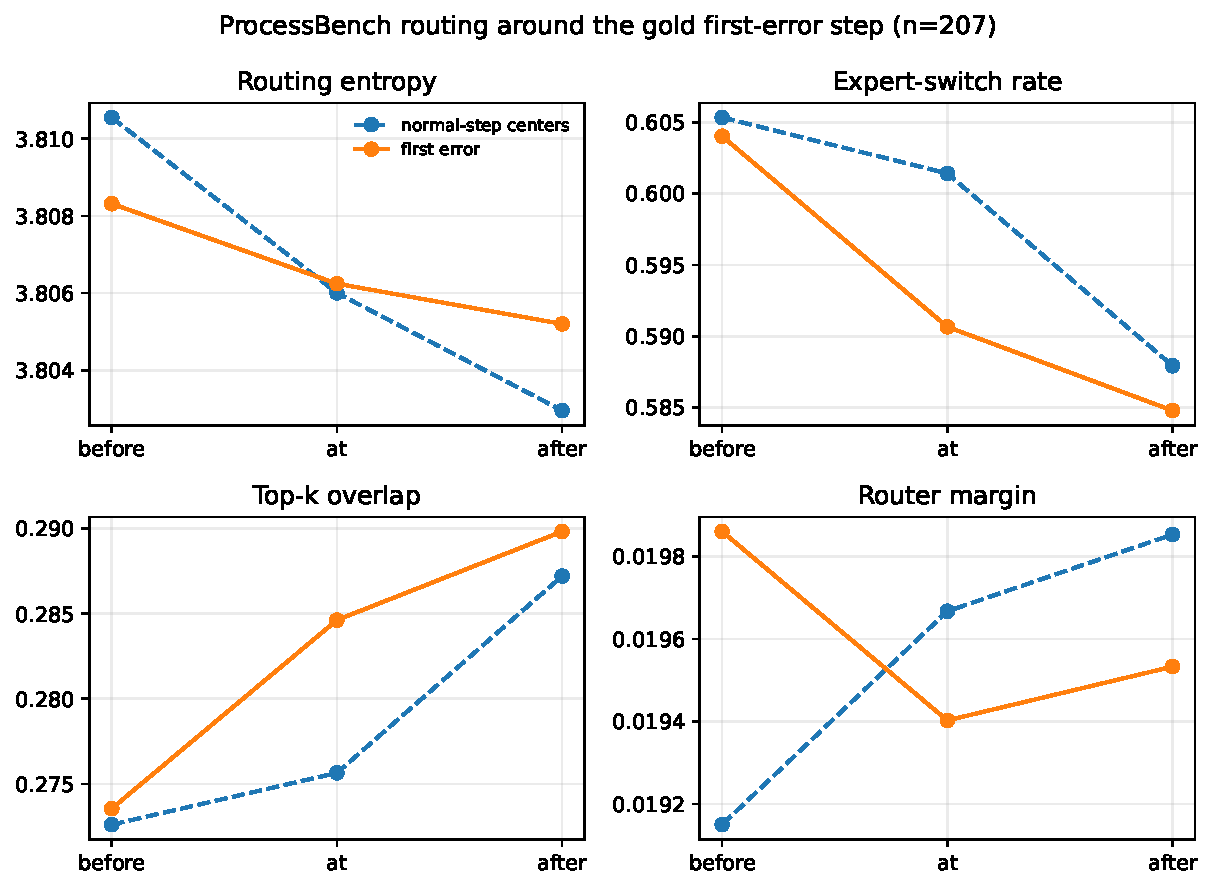
\includegraphics[width=0.82\textwidth]{paper_figures/processbench_first_error_routing.pdf}
\caption{Before/at/after trajectories for ProcessBench gold first errors and
normal-step centers.  The visual differences are descriptive; the controlled
effects in Table~\ref{tab:first-error-control} are not statistically resolved.}
\label{fig:first-error-routing}
\end{figure*}

Plain GSM8K still has only two event-eligible traces, so its event effects are
case studies.  Self-checking increases GSM8K coverage to ten eligible traces,
but every bootstrap interval for backtracking, self-correction, and the first
detected event contains zero.  Table~\ref{tab:generated-routing} summarizes
the better-powered generated-data comparisons.  Two small MATH entropy
effects are resolved: contradiction in the baseline condition and the first
detected event under self-checking.  In MATH self-check backtracking/
self-correction spans, the router margin falls.  The latter labels identify
the same nine traces and nearly the same spans, so they are not independent
replications.  None of these analyses corrects for the many event--metric
comparisons, and trace counts are only 9--24; they are exploratory rather than
evidence of a universal event signature.

\begin{table*}[t]
\centering
\caption{Current generated-data matched-control effects. Values are event
change minus change at a matched normal position; intervals are trace-level
95\% bootstrap intervals with 2,000 replicates.  \modelmetrics{
\texttt{allenai/OLMoE-1B-7B-0924-Instruct}}{eligible-trace count and mean
matched-control differences in routing entropy, top-$k$ switch rate, top-$k$
Jaccard overlap, and router margin, each with a 95\% confidence interval}}
\label{tab:generated-routing}
\resizebox{\textwidth}{!}{%
\begin{tabular}{llrrrrr}
\toprule
Condition & Event & $n$ & $\Delta$ entropy & $\Delta$ switch & $\Delta$ overlap & $\Delta$ margin \\
\midrule
GSM8K + self-check & Backtracking & 9 & $-0.00670$ $[-0.04040,0.03064]$ & $0.01237$ $[-0.06946,0.09246]$ & $-0.00226$ $[-0.07058,0.06825]$ & $-0.000833$ $[-0.004740,0.003242]$ \\
GSM8K + self-check & Self-correction & 7 & $-0.01062$ $[-0.05124,0.03238]$ & $0.03934$ $[-0.02679,0.11244]$ & $-0.02583$ $[-0.10064,0.03729]$ & $-0.000534$ $[-0.005338,0.004480]$ \\
MATH & Contradiction & 15 & $0.04381$ $[0.01039,0.07702]$ & $0.02031$ $[-0.06303,0.10522]$ & $-0.01834$ $[-0.09607,0.06839]$ & $-0.000884$ $[-0.005099,0.003685]$ \\
MATH + self-check & First detected event & 24 & $0.04130$ $[0.00639,0.07399]$ & $0.03743$ $[-0.03776,0.10645]$ & $-0.02995$ $[-0.09325,0.03043]$ & $-0.002898$ $[-0.005988,0.000365]$ \\
MATH + self-check & Backtracking & 9 & $0.03671$ $[-0.02635,0.09093]$ & $0.04991$ $[-0.04862,0.13413]$ & $-0.04524$ $[-0.11074,0.03742]$ & $-0.003962$ $[-0.007604,-0.000631]$ \\
\bottomrule
\end{tabular}}
\end{table*}

The retained corrected PRM800K output contains 4,315 gold first-error traces,
87 traces with explicit contradictions, and 89 first heuristic reasoning
events.  Table~\ref{tab:prm-routing} reports its earlier matched analysis.
Contradiction and first-event intervals include zero.  At the gold first
error, switching falls, overlap rises, and margin rises by small amounts.  It
is a useful counterexample to a universal disruption hypothesis, but it is
legacy evidence: the current PRM800K pipeline did not regenerate it.

\begin{table*}[t]
\centering
\caption{Legacy corrected PRM800K matched-control effects at the event.
Intervals are trace-level 95\% bootstrap intervals with 1,000 replicates.
\modelmetrics{\texttt{allenai/OLMoE-1B-7B-0924-Instruct}, legacy PRM800K
run}{eligible-trace count and mean matched-control differences in routing
entropy, top-$k$ switch rate, top-$k$ Jaccard overlap, and router margin, each
with a 95\% confidence interval}}
\label{tab:prm-routing}
\resizebox{\textwidth}{!}{%
\begin{tabular}{lrrrrr}
\toprule
Event & $n$ traces & $\Delta$ entropy & $\Delta$ switch & $\Delta$ overlap & $\Delta$ margin \\
\midrule
Contradiction & 87 & $-0.00210$ $[-0.02381,0.01722]$ & $0.00576$ $[-0.03197,0.04148]$ & $-0.00324$ $[-0.03431,0.02971]$ & $0.000146$ $[-0.001789,0.002247]$ \\
First reasoning event & 89 & $-0.00491$ $[-0.02597,0.01449]$ & $0.00888$ $[-0.02478,0.04288]$ & $-0.00637$ $[-0.03866,0.02663]$ & $0.000511$ $[-0.001572,0.002594]$ \\
Gold first error & 4,315 & $-0.00187$ $[-0.00485,0.00107]$ & $-0.02120$ $[-0.02687,-0.01577]$ & $0.01980$ $[0.01457,0.02515]$ & $0.000474$ $[0.000158,0.000801]$ \\
\bottomrule
\end{tabular}}
\end{table*}

Legacy PRM800K backtracking ($n=2$) and self-correction ($n=1$) remain case
studies and are omitted from the inferential table.

\subsection{Hidden-state geometry and routing}

For each layer, we compute the pairwise cosine-similarity matrix of sampled
token hidden states and the cosine-similarity matrix of their softmax router
distributions.  Their upper triangles are correlated; the overall
significance test is a 1,000-permutation Mantel test.  This is a geometry--
routing correlation analysis, not t-SNE and not a linear-separability probe.
The exposed hidden state is the input to the transformer layer and is the
closest available proxy for, but not exactly, the post-attention state seen by
that layer's router.

Figure~\ref{fig:geometry} and Table~\ref{tab:geometry-summary} show the most
replicated result in the study.  Mean overall correlation lies in the narrow
range 0.5605--0.5663 across all five current conditions.  It rises sharply
from layer 0 and peaks in layer 3 or 4 before declining moderately.  Every
layer in every condition reaches the permutation-resolution floor
$p=1/1001\approx0.000999$.

\begin{figure*}[t]
\centering
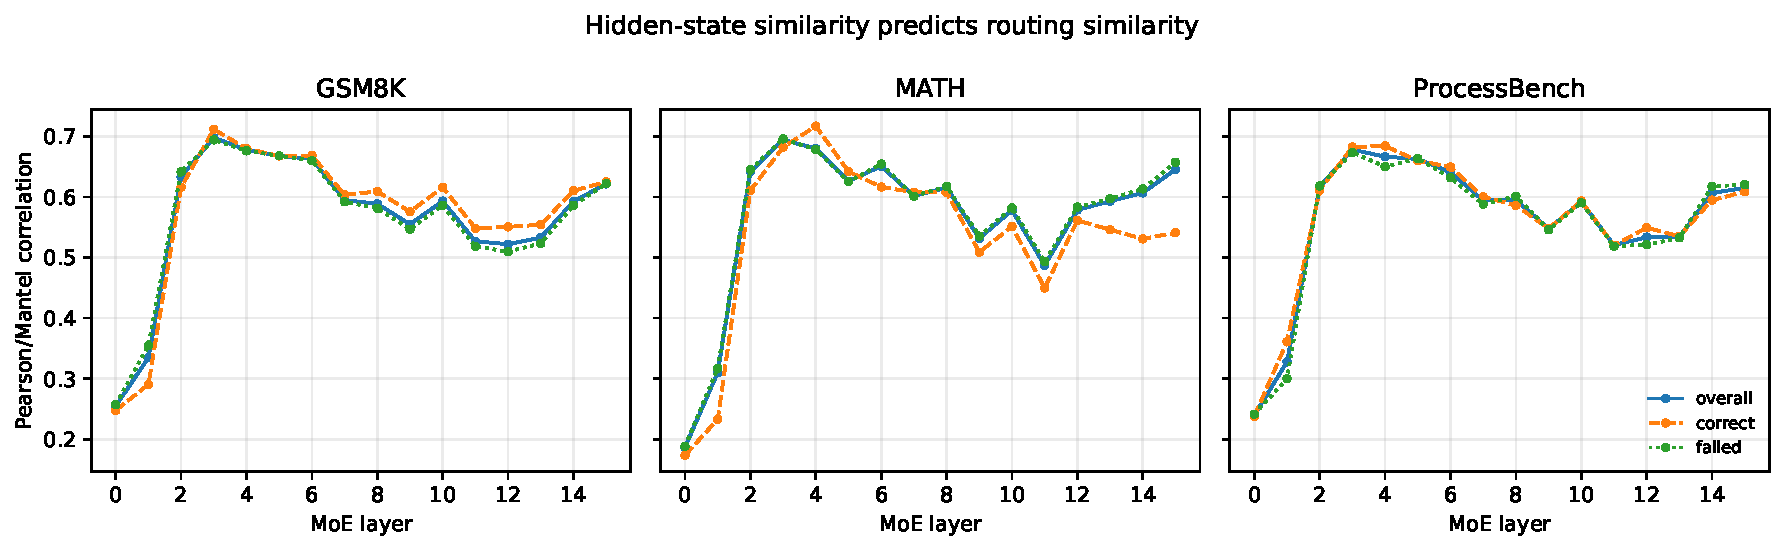
\includegraphics[width=0.96\textwidth]{paper_figures/geometry_correlation.pdf}
\caption{Layerwise correlation between hidden-state similarity and routing-
distribution similarity for three representative current conditions.}
\label{fig:geometry}
\end{figure*}

\begin{table*}[t]
\centering
\caption{Summary of geometry--routing correlations across 16 layers.
\modelmetrics{\texttt{allenai/OLMoE-1B-7B-0924-Instruct}}{Pearson correlation
between the upper triangles of hidden-state and router-distribution pairwise
cosine-similarity matrices; the table gives the layer mean, layer range, peak
layer, and correct- versus failed-subset means}}
\label{tab:geometry-summary}
\resizebox{\textwidth}{!}{%
\begin{tabular}{lrrrrr}
\toprule
Condition & Overall mean & Overall range & Peak layer & Correct mean & Failed mean \\
\midrule
GSM8K & 0.5659 & 0.2550--0.6977 & 3 & 0.5732 & 0.5635 \\
GSM8K + self-check & 0.5644 & 0.2529--0.6936 & 3 & 0.5830 & 0.5597 \\
MATH & 0.5641 & 0.1870--0.6940 & 3 & 0.5360 & 0.5676 \\
MATH + self-check & 0.5663 & 0.2194--0.6809 & 4 & 0.5655 & 0.5684 \\
ProcessBench & 0.5605 & 0.2399--0.6779 & 3 & 0.5637 & 0.5570 \\
\bottomrule
\end{tabular}}
\end{table*}

Correct-versus-failed differences are inconsistent.  Correct traces have the
higher mean on GSM8K, GSM8K self-check, and ProcessBench; failed traces have
the higher mean on MATH and (slightly) MATH self-check.  No trace-bootstrap
interval is available for these contrasts.  The overall analysis uniformly
samples 1,000 tokens per condition and the Mantel permutation treats sampled
tokens as exchangeable; it does not provide trace-level uncertainty or prove
that representations cause routing.  The defensible conclusion is narrower:
hidden-state and router-distribution geometries are strongly aligned and the
layerwise profile replicates across datasets and prompts, while outcome
modulation does not.

\subsection{Prospective prefix probes}

Experiment~4 now supplies the prospective test that was previously missing.
Table~\ref{tab:prospective-final} reports early (25\%) and late (75\%) prefixes;
the omitted 50\% results lie between them except where noted below.  On GSM8K
and both MATH conditions, a three-feature length/step/character baseline is as
good as or better than router, hidden, and combined representations at most
prefixes.  MATH is especially clear: structure AUROC is approximately 0.763--
0.774 while the best representation probe reaches at most 0.745.  This makes
trace structure a major confound, not merely a weak baseline.

\begin{table*}[t]
\centering
\caption{Prospective final-incorrectness AUROC from prefix-only features.
Representation entries select the best of 16 layers (shown in parentheses),
so their comparison is exploratory and selection-optimistic.  ``Positive''
is the number of finally incorrect traces.  \modelmetrics{
\texttt{allenai/OLMoE-1B-7B-0924-Instruct}, with trace-grouped logistic
probes}{prefix fraction, trace and positive counts, and out-of-fold AUROC for
structure-only, router-only, hidden-only, and combined features; parentheses
give the selected layer}}
\label{tab:prospective-final}
\resizebox{\textwidth}{!}{%
\begin{tabular}{lrrrrrrr}
\toprule
Condition & Prefix & $N$ & Positive & Structure & Router & Hidden & Combined \\
\midrule
GSM8K & 25\% & 1,319 & 826 & 0.6819 & 0.6512 (L10) & 0.6559 (L12) & 0.6514 (L10) \\
       & 75\% & 1,319 & 826 & 0.6819 & 0.6887 (L13) & 0.6839 (L12) & 0.6830 (L8) \\
GSM8K + self-check & 25\% & 1,319 & 844 & 0.6960 & 0.6732 (L7) & 0.6880 (L9) & 0.6874 (L10) \\
       & 75\% & 1,319 & 844 & 0.6959 & 0.6843 (L9) & 0.7070 (L10) & 0.7105 (L10) \\
MATH & 25\% & 1,499 & 1,297 & 0.7628 & 0.7144 (L12) & 0.7189 (L14) & 0.7252 (L14) \\
     & 75\% & 1,499 & 1,297 & 0.7628 & 0.7319 (L10) & 0.7445 (L12) & 0.7370 (L6) \\
MATH + self-check & 25\% & 1,500 & 1,323 & 0.7736 & 0.7118 (L10) & 0.7216 (L14) & 0.7112 (L14) \\
     & 75\% & 1,500 & 1,323 & 0.7735 & 0.7446 (L10) & 0.7420 (L15) & 0.7402 (L15) \\
ProcessBench & 25\% & 400 & 207 & 0.6192 & 0.6267 (L9) & 0.6171 (L7) & 0.6171 (L6) \\
             & 75\% & 400 & 207 & 0.6184 & 0.6685 (L4) & 0.6931 (L11) & 0.7022 (L11) \\
\bottomrule
\end{tabular}}
\end{table*}

ProcessBench is the exception for final incorrectness: combined AUROC rises
from 0.617 at 25\% to 0.702 at 75\%, versus a 0.618 structure baseline.  The
signal therefore emerges after much of the solution is visible, which is
useful for monitoring but weaker evidence of advance prediction.

The stricter future-first-error target is available only on ProcessBench.
At 25\%, combined features reach AUROC 0.674 (95\% bootstrap CI
$[0.612,0.733]$) versus 0.625 for structure.  This advantage disappears at
50\%, where structure is 0.640 and combined features are 0.563.  At 75\%,
only 13 future errors remain; the best router AUROC is 0.682 with the very
wide interval $[0.535,0.832]$.  Fractions condition on the error not having
occurred yet, so their populations and class prevalence differ and should
not be read as a learning curve.  Together with best-layer selection and the
absence of paired model-comparison tests, these results do not establish a
robust advance failure detector.

\subsection{Expert usage by reasoning phase}

Experiment 5 measures each expert's activation frequency and weight mass by
phase, before/after event usage, co-activation, and top-1 transition matrices.
The outputs in Table~\ref{tab:expert-phase} and Figure~\ref{fig:expert-phase}
use current labels.  Each cell reports the mean absolute activation-frequency
difference over all $16\times64$ layer--expert cells relative to normal
tokens, followed by the number of phase tokens.  Token counts are not numbers
of independent traces; in particular, explicit event phases remain supported
by only 1--9 traces per condition.

\begin{table*}[t]
\centering
\caption{Expert-activation shifts relative to normal tokens. Parentheses give
phase-token counts; a dash indicates no tokens for that phase.
\modelmetrics{\texttt{allenai/OLMoE-1B-7B-0924-Instruct}}{mean absolute
activation-frequency difference from normal tokens across all
$16\times64$ layer--expert cells, plus phase-token counts}}
\label{tab:expert-phase}
\resizebox{\textwidth}{!}{%
\begin{tabular}{lrrrrr}
\toprule
Dataset & Backtrack & Contradiction & Self-correction & First error & Final answer \\
\midrule
GSM8K & 0.0608 (61) & 0.0804 (82) & 0.0608 (61) & -- & 0.0136 (139,075) \\
GSM8K + self-check & 0.0266 (2,512) & 0.0390 (670) & 0.0303 (1,997) & -- & 0.0129 (70,550) \\
MATH & -- & 0.0224 (1,677) & -- & -- & 0.0160 (167,642) \\
MATH + self-check & 0.0175 (2,345) & 0.0154 (4,085) & 0.0175 (2,345) & -- & 0.0143 (119,763) \\
ProcessBench & 0.0592 (162) & -- & 0.0592 (162) & 0.0104 (14,539) & 0.0185 (13,210) \\
\bottomrule
\end{tabular}}
\end{table*}

\begin{figure*}[t]
\centering
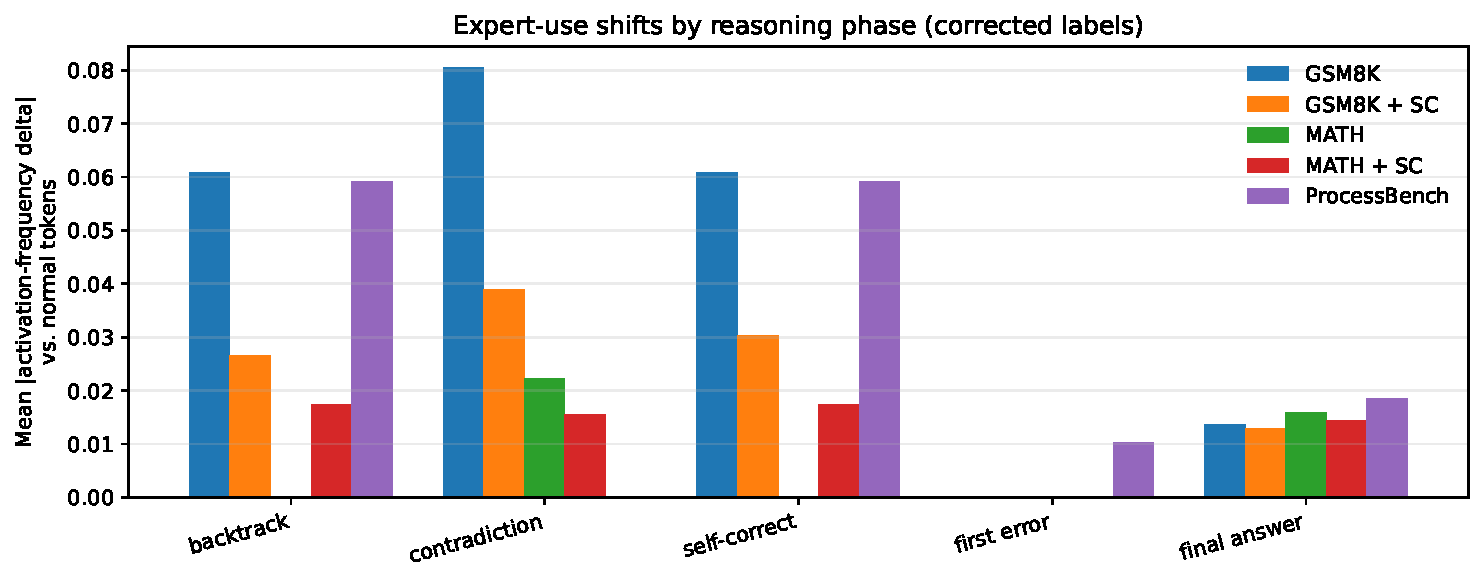
\includegraphics[width=0.78\textwidth]{paper_figures/expert_phase_deltas.pdf}
\caption{Mean absolute expert-activation-frequency shift by reasoning phase.
Explicit backtracking/self-correction bars have very small trace counts even
when they contain many tokens.}
\label{fig:expert-phase}
\end{figure*}

The reliable ProcessBench first-error phase has only a 0.0104 mean absolute
shift from normal expert frequencies.  Comparing the five tokens after each
gold first error with the five before it gives a mean absolute layer--expert
change of 0.0139 over 207 events; the largest cell change is 0.0879.  For the
self-check conditions, five-token before/after changes at self-corrections are
0.0521 over ten GSM8K event occurrences and 0.0436 over ten MATH occurrences,
but every associated trace ends incorrect and no matched-control interval is
available.  These are state changes around failed revision attempts, not
evidence of recovery experts.

Table~\ref{tab:transition-persistence} adds the marginal-frequency baseline
missing from the preliminary analysis.  For each layer, the baseline is the
self-transition probability under independent source and destination draws
with the observed marginals, then pooled by transition count.  Observed
persistence is 9--10 percentage points above this baseline in every current
condition.  The effect is descriptive---there is no trace-level uncertainty
and token identity/content are uncontrolled---but it does show that the
roughly 19--30\% self-transition shares are not explained solely by expert
imbalance.

\begin{table}[t]
\centering
\caption{Global top-1 expert transition persistence and a marginal-frequency
independence baseline.  \modelmetrics{
\texttt{allenai/OLMoE-1B-7B-0924-Instruct}}{adjacent-token transition count,
observed top-1 self-transition percentage, and expected self-transition
percentage under independent source/destination draws with observed
marginals}}
\label{tab:transition-persistence}
\begin{tabular}{lrrr}
\toprule
Condition & Transitions & Self-transition & Independence \\
\midrule
GSM8K & 5,398,816 & 19.79\% & 9.90\% \\
GSM8K + self-check & 5,456,304 & 19.30\% & 9.82\% \\
MATH & 10,396,432 & 29.86\% & 20.58\% \\
MATH + self-check & 10,390,832 & 29.49\% & 20.14\% \\
ProcessBench & 1,681,792 & 20.54\% & 10.19\% \\
\bottomrule
\end{tabular}
\end{table}

\subsection{Qwen MATH-500 correlation experiment}

The correlation pipeline completed all 500 MATH-500 problems with one sampled
trace per problem.  Qwen3.5-35B-A3B answered 387 correctly (77.4\%).  The
lexical detectors marked 133 traces with backtracking, 97 with
self-correction, and 70 with contradiction.  The analysis contains 59 trace
features, including prespecified summaries across the six router layers
selected by the independent Schoenfeld probe run.  Table~\ref{tab:qwen-corr}
reports point-biserial correlations; intervals resample source problems.
Because there is exactly one trace per problem, the 500 bootstrap clusters are
also the 500 observations.

\begin{table*}[t]
\centering
\caption{Prespecified Qwen MATH-500 trace-level correlations.  Positive $r$
means larger feature values in traces for which the binary target is present.
Intervals are 95\% problem-cluster bootstrap intervals.
\modelmetrics{Qwen3.5-35B-A3B (\texttt{UD-Q4\_K\_XL} GGUF generation and
matching \texttt{unsloth/Qwen3.5-35B-A3B} routing replay with runtime 4-bit
quantization)}{point-biserial $r$ between each binary trace target and the
listed continuous feature, with problem-cluster bootstrap 95\% confidence
intervals}}
\label{tab:qwen-corr}
\begin{tabular}{llrr}
\toprule
Target & Feature & $r$ & 95\% CI \\
\midrule
Correct answer & Mean router entropy & $-0.555$ & $[-0.614,-0.500]$ \\
Correct answer & Token count & $-0.520$ & $[-0.562,-0.480]$ \\
Correct answer & Mean hidden-state norm & $-0.488$ & $[-0.554,-0.419]$ \\
Correct answer & Mean router margin & $0.301$ & $[0.231,0.376]$ \\
Correct answer & Mean hidden/router geometry & $-0.238$ & $[-0.307,-0.164]$ \\
Backtracking & Token count & $0.453$ & $[0.399,0.501]$ \\
Backtracking & Mean router entropy & $0.364$ & $[0.268,0.452]$ \\
Self-correction & Token count & $0.382$ & $[0.336,0.429]$ \\
Self-correction & Mean router entropy & $0.325$ & $[0.224,0.411]$ \\
Contradiction & Mean hidden-state norm & $0.329$ & $[0.259,0.393]$ \\
Contradiction & Token count & $0.247$ & $[0.189,0.302]$ \\
\bottomrule
\end{tabular}
\end{table*}

Correct traces are shorter and exhibit lower mean router entropy, smaller
hidden-state norms and trajectory steps, less top-1 switching, greater top-$k$
overlap, and larger router margins.  The entropy association is the largest
prespecified routing result.  Exploratory layerwise screening yields similar
or slightly larger magnitudes---entropy at layer 27 has $r=-0.574$, and
hidden-state step distance at layer 39 has $r=-0.572$---but these maxima do not
have selection-adjusted intervals and should not be treated as confirmed
layer localization.

The same direction recurs for the lexical reasoning-event targets: traces
with backtracking or self-correction tend to be longer, higher-entropy, and
lower-margin.  However, token count is itself strongly associated with
correctness and is the largest correlate of backtracking and self-correction.
The present analysis reports marginal correlations and does not condition
routing features on length, problem difficulty, or token content.  It
therefore cannot distinguish a routing-specific signal from longer or harder
failed solutions having more opportunities for revision markers and different
activation statistics.  With one attempt per problem, problem-level pass-rate
correlations and within-problem correct-minus-incorrect contrasts are empty;
the repeated-attempt design is required for those stronger controls.

\subsection{Legacy full-trace linear routing probes}

Before the current prospective run, we trained a separate linear logistic
probe at each layer using one pooled
router-feature vector per trace.  The 197 features comprise router-probability
means and standard deviations, top-1 expert frequencies, entropy and margin
statistics, and top-1 switch rate.  Five-fold stratified cross-validation
produces out-of-fold predictions; 95\% intervals bootstrap traces.  Since each
trace contributes one sample, token leakage across folds is impossible.  The
probe pools the \emph{complete} trace, so this is a decoding/separability test,
not online prediction of a future error.  These files are retained because
they include the only nonempty PRM800K probe, but the GSM8K generations and
labels are not identical to the current run; they are not compared numerically
with Table~\ref{tab:prospective-final}.

\begin{figure*}[t]
\centering
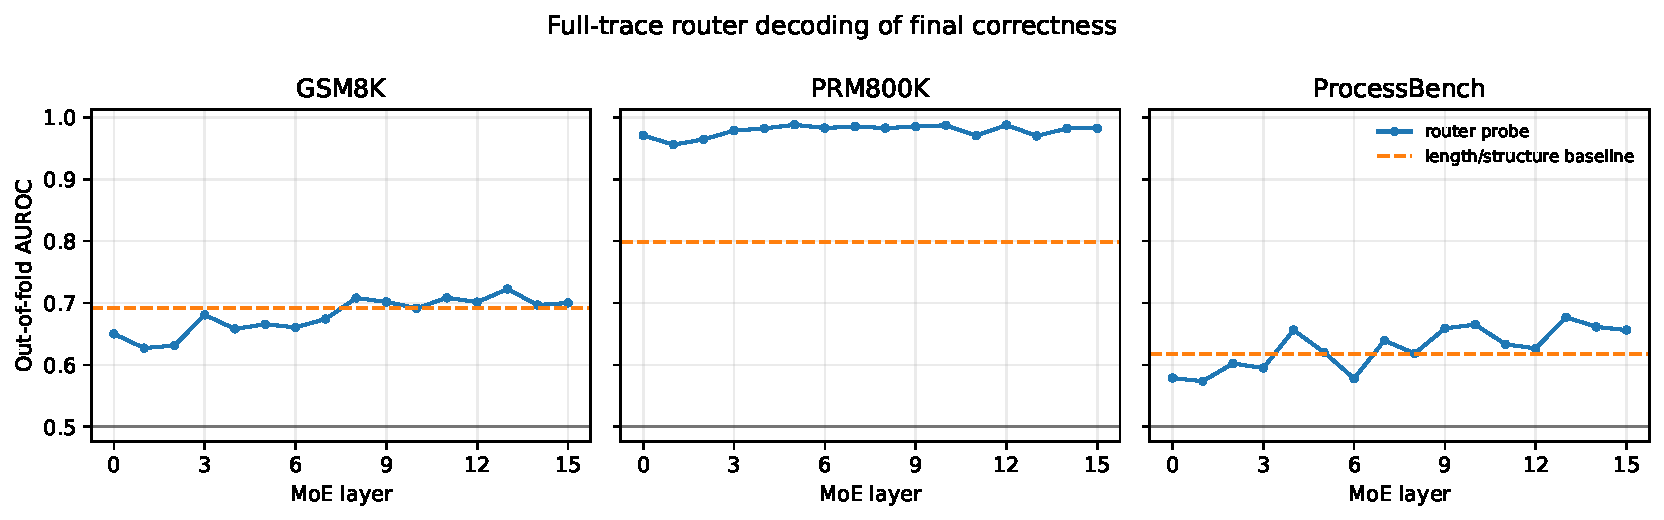
\includegraphics[width=0.96\textwidth]{paper_figures/router_correctness_probes.pdf}
\caption{Out-of-fold correctness AUROC by layer. Dashed lines use only log
token count, log step count, and log character count.}
\label{fig:router-probes}
\end{figure*}

\begin{table*}[t]
\centering
\caption{Legacy best-layer full-trace router probes. The selected-layer
comparison is exploratory and is not corrected for selecting the best of 16
layers.  \modelmetrics{\texttt{allenai/OLMoE-1B-7B-0924-Instruct}, with
five-fold trace-level logistic probes; PRM800K is legacy}{trace and positive
counts, selected layer, out-of-fold router-feature AUROC with trace-bootstrap
95\% confidence interval, balanced accuracy, and structure-baseline AUROC}}
\label{tab:router-probes}
\resizebox{\textwidth}{!}{%
\begin{tabular}{llrrrrrr}
\toprule
Dataset & Target & $N$ & Positive & Best layer & Router AUROC [95\% CI] & Balanced acc. & Structure AUROC \\
\midrule
GSM8K & Correctness & 1,319 & 486 & 13 & 0.7225 $[0.6944,0.7505]$ & 0.6655 & 0.6917 \\
PRM800K & Correctness & 10,833 & 6,518 & 5 & 0.9882 $[0.9858,0.9905]$ & 0.9760 & 0.7981 \\
PRM800K & Gold first error & 10,833 & 4,315 & 5 & 0.9882 $[0.9857,0.9904]$ & 0.9760 & 0.7981 \\
PRM800K & Contradiction & 10,833 & 87 & 9 & 0.9082 $[0.8702,0.9385]$ & 0.7489 & 0.7573 \\
ProcessBench & Correctness & 400 & 193 & 13 & 0.6771 $[0.6244,0.7272]$ & 0.6356 & 0.6181 \\
ProcessBench & Gold first error & 400 & 207 & 13 & 0.6771 $[0.6240,0.7303]$ & 0.6356 & 0.6181 \\
\bottomrule
\end{tabular}}
\end{table*}

Routing improves over the simple structure baseline by 0.031 AUROC on GSM8K,
0.190 on PRM800K correctness/first-error, 0.151 on PRM800K contradiction, and
0.059 on ProcessBench.  PRM800K correctness and first-error scores are the same
because, in these traces, presence of a gold first error is the complement of
the final correctness label.  The contradiction AUROC is high despite only 87
positives, but F1 at the AUROC-selected layer is only 0.159 under the natural
class imbalance.  Backtracking and self-correction probes were correctly
skipped: their positive counts after relabelling are 1/1 on GSM8K, 2/1 on
PRM800K, and 3/3 on ProcessBench.

The near-perfect PRM800K correctness AUROC (0.988) should be treated with
particular caution.  The probe sees the complete provided solution, the first-
error target is exactly complementary to correctness in this output, and
source/format artifacts can be encoded in pooled routing statistics.  The
current zero-input PRM800K failure prevents a prefix-only hidden/router check,
so this result establishes legacy within-file decodability only.

\section{Analysis}

\subsection{Conclusions supported so far}

\begin{enumerate}
\item Hidden-state geometry strongly predicts router-distribution geometry at
every layer in all five current conditions.  Overall mean correlation is
0.5605--0.5663, peaks in layer 3 or 4, and is nearly invariant to self-check
prompting.  Correct--failed differences reverse direction across conditions.
\item At 207 gold ProcessBench first errors, entropy, switching, overlap, and
margin do not exhibit a statistically resolved discontinuity relative to a
matched position in the same trace.  Simple layer-averaged routing metrics are
therefore not sufficient first-error markers in the current analysis.
\item Self-check prompting increases explicit revision markers but does not
improve final accuracy on paired GSM8K or MATH problems.  Every trace labelled
as a self-correction in the two self-check conditions ends incorrect.
\item MATH exhibits a small entropy increase at detected reasoning events,
and MATH self-check backtracking spans exhibit a small margin decrease.  These
effects use only 9--24 traces, are uncorrected for multiple comparisons, and
do not replicate as a universal multi-metric disruption.
\item Prospective final-incorrectness probes are usually matched or beaten by
the structure baseline on GSM8K and MATH.  ProcessBench combined features
reach AUROC 0.702 at 75\%, but its 25\% future-first-error result is only 0.674
and the signal is not stable across later conditional cohorts.  A robust
advance detector has not been established.
\item Top-1 routes persist more than a marginal-frequency independence
baseline in every current condition, but event-specific expert shifts remain
descriptive and explicit-event trace counts remain small.
\item In the completed 500-problem Qwen MATH-500 correlation run, correctness
is associated with lower mean router entropy ($r=-0.555$, 95\% CI
$[-0.614,-0.500]$) and larger mean router margin ($r=0.301$,
$[0.231,0.376]$).  Correct traces are also substantially shorter
($r=-0.520$), while backtracking and self-correction are most strongly
associated with greater length.  These are marginal trace-level associations;
the current single-attempt design cannot isolate routing from length or
problem difficulty.
\item The auxiliary Qwen3.5 boundary probes show substantial sentence-split
decodability of upcoming Schoenfeld episodes (selected-layer AUROC
0.835--0.934), with the strongest thresholded results for Implement, Verify,
and Read.  This establishes accessible prefix-state signal within familiar
responses, not generalization to unseen reasoning traces.
\item External application of the episode probes is best interpreted as
coarse phase inspection.  Predictions collapse toward Implement, Read, and
Monitor; Explore is never selected and 12.7\% of units activate no probe.  A
provisional hybrid pragmatic review gives 50.3\% strict and 60.8\% compatible
agreement, with 187/581 multi-label units.  Implement is strongest (F1 0.729),
whereas Analyze, Plan, Explore, Verify, and Monitor remain incomplete external
tags.  ProcessBench Verify predictions identify review-heavy passages after
errors but do not identify correctness.
\item The current PRM800K run failed with zero input despite completion
banners.  Its earlier first-error stabilization and near-perfect full-trace
decoding results are legacy evidence and require a clean prospective rerun.
\end{enumerate}

\subsection{What has not been established}

The present experiments do not identify ``math experts'' or ``failure
experts'', do not show that routing changes cause reasoning errors, and do not
show that backtracking forms a stable, linearly separable hidden-state class.
Hidden and combined prefix probes have now been run, but their advantage over
structure is inconsistent and best-layer comparisons are selection-optimistic.
No t-SNE/UMAP visualization or routing intervention has been run.  The
geometry significance test does not supply trace-level uncertainty, event
analyses are not multiplicity-corrected, and the expert transition baseline
does not control token content.  Correlation and linear decodability should
not be read as causal evidence.  The Schoenfeld boundary-probe run also does
not establish response-grouped generalization, calibrated seven-way episode
classification, or the cognitive states of Qwen's own generations.  It uses
Qwen to encode teacher-forced DeepSeek-R1 text, shares all 38 response IDs
between train and test, and selects layers on the reported test set.  Its
external argmax outputs have no authoritative human or benchmark episode
ground truth.  Agreement with the provisional hybrid review is diagnostic and
should not be called validated transfer accuracy.  The Qwen MATH-500
correlations likewise do not establish an independent routing predictor or a
causal mechanism: no length-conditioned model has been fit, only one attempt
is available per problem, and the other planned benchmarks have not yet been
analyzed.  Layerwise maxima are exploratory comparisons without
selection-adjusted uncertainty.

\section{Discussion}

The strongest current story remains geometry-first: routing follows the
evolving representation space, with a consistent layerwise signature across
five dataset and prompt conditions.  The anticipated universal sharp disruption
at errors is not supported.  ProcessBench is null at the gold first error,
MATH has a selective entropy increase at heuristically detected events, and
legacy PRM800K shows a small stabilization.  Direction and metric therefore
depend on the dataset and event definition.

The prospective runs also change the interpretation of decodability.  Much of
final-incorrectness prediction on generated math traces is already present in
prefix length and structure; representation features add most clearly only
late in ProcessBench.  Future work should use paired model comparisons,
prespecified layers, trace-level uncertainty, and targets defined strictly
after the observed prefix.  A clean PRM800K rerun is necessary before treating
its unusually high legacy decoding score as a model-level phenomenon.

The Qwen MATH-500 run reinforces this structural caution on a larger model.
Lower entropy and higher margin accompany correct answers, but incorrect and
revision-bearing traces are also longer.  The appropriate next test is the
planned repeated-attempt analysis: compare correct and incorrect samples of
the same problem, condition on trace length and token composition, and check
whether the aggregate entropy and margin effects replicate across datasets.

The auxiliary episode probes add a complementary representation-level result:
the prefix before a sentence often encodes the phase likely to follow, and the
signal is strongest in middle-to-late layers rather than at the final model
output.  The current split cannot determine whether this reflects a portable
episode representation, trace-specific transition regularities, position, or
formatting.  A response-grouped nested evaluation should select both layer and
regularization on inner folds, evaluate once on unseen responses, repeat over
seeds, and report response-bootstrap intervals.  Standardized or norm-matched
features and simple position/previous-unit/format baselines are needed to
separate hidden-state information from layer scale and trace structure.

For external use, the probe outputs should be treated as abstaining phase
suggestions rather than annotations.  Abbreviation- and LaTeX-aware
segmentation should precede evaluation; independent one-versus-rest scores
should either be calibrated on a common multiclass validation set or retain
multiple labels.  The pragmatic review confirms substantial ambiguity and
only 60.8\% compatible agreement; independent human annotators should resolve
the 37 low-confidence units and assess inter-annotator agreement before any
transfer-accuracy claim.  It would also be useful to
separate cross-model recognition, as studied here, from Qwen's own generation
by running the same protocol on Qwen-generated traces.

The event-label audit also changes the experimental priority.  Explicit
lexical markers provide high precision but extremely low recall.  Robust
backtracking conclusions will require either deliberately elicited
self-checking traces, manual/LLM-assisted span annotation with validation, or
a benchmark with revision spans.  Until then, the gold ProcessBench error
analysis and outcome-based correct/failed comparisons are the safest results.

\section{Conclusion}

OLMoE routing is strongly and reproducibly aligned with hidden-state geometry,
but aggregate metrics do not provide a dataset-invariant error signature.
Self-check prompting elicits more revision language without improving paired
accuracy, and prospective representation probes seldom beat simple structure
baselines on generated math.  ProcessBench shows a moderate late-prefix
signal but no resolved discontinuity at its gold first error.  Expert routes
are more persistent than their marginal frequencies predict, yet event-
specific expert claims remain underpowered.  The auxiliary episode-judge study
likewise favors conservative conclusions.  Static-reward, context-aware
light-budget GEPA reaches 0.650 cross-validated macro-F1, with only a small
advantage over the prior selector and worse performance under the heavy search.
The completed same-model LLM-judge final fit raises development-set balanced
accuracy from 0.677 to 0.777 and macro-F1 from 0.613 to 0.727, primarily by
reducing Monitor overprediction, but it selects among 145 candidates on those
same six responses and does not evaluate the locked test.  This is
prompt-optimization evidence rather than a generalization estimate.  The separate
Qwen3.5 boundary probes
show strong within-split linear access to upcoming episode labels, especially
for Implement, Verify, and Read, but their sentence split leaks every response
across train and test and their external outputs collapse to a coarse
setup/execution/review taxonomy.  Provisional pragmatic adjudication yields
50.3\% primary and 60.8\% compatible agreement; only Implement transfers
strongly at class level (F1 0.729), and 32.2\% of units admit two defensible
labels.  They therefore support prospective
within-trace phase decodability, not unseen-trace generalization, automatic
seven-way annotation, error detection, or claims about Qwen's own generated
cognition.  The next priorities are a clean PRM800K rerun, adjudication of
episode-unit artifacts, paired seed-versus-GEPA outer evaluation,
response-grouped nested boundary probes with validated external labels,
stronger event supervision, and only then causal routing intervention.
The new Qwen MATH-500 result adds a robust descriptive association---correct
traces have lower router entropy and higher margin---but its co-occurring
length effects and single-attempt design prevent an independent or causal
routing claim.  Completing the repeated-attempt benchmarks and within-problem
contrasts is the immediate requirement for that line of evidence.

\appendix

\section{Reproducibility Checklist}

\begin{table*}[h]
\centering
\scriptsize
\caption{Living inventory of completed and pending work.
\modelmetrics{All models in the report: Qwen3.6-27B \texttt{Q4\_K\_XL},
\texttt{Qwen/Qwen3.5-35B-A3B-GPTQ-Int4}, Qwen3.5-35B-A3B correlation-run
variants, and \texttt{allenai/OLMoE-1B-7B-0924-Instruct}}{workflow status,
run/sample counts, and selected headline metrics stated per row; this is an
inventory rather than a common-metric evaluation}}
\label{tab:status}
\begin{tabular}{p{0.22\textwidth}p{0.13\textwidth}p{0.55\textwidth}}
\toprule
Item & Status & Note / next action \\
\midrule
Trace generation / ingestion & Partial & Current: GSM8K and GSM8K self-check 1,319 each; MATH and MATH self-check 1,500 each; ProcessBench 400. PRM800K is zero-byte and must be rerun. \\
Router/hidden extraction & Done for five conditions & All five non-PRM JSONL files validate and have complete router/hidden tensors; PRM800K current output is empty. \\
High-precision labels & Done/current & Current five-condition outputs use the conservative classifier; legacy PRM800K has a separate corrected-label file. \\
Taxonomy summary file & Done/current & \texttt{results/exp1/summary.json} contains the five current conditions; corrected legacy PRM800K remains in \texttt{summary\_relabelled.json}. \\
ProcessBench event routing & Done/current & Gold first error has matched controls and 2,000-sample bootstrap CIs. \\
Generated-data event routing & Done but underpowered & Plain/self-check GSM8K and MATH are complete; event-eligible trace counts range from 2 to 24. \\
PRM800K event routing & Legacy only & Corrected earlier output covers 4,371 event-eligible traces; current zero-input run did not reproduce it. \\
Geometry--routing correlation & Done for five conditions & Overall/correct/failed and current-label backtracking outputs exist for every non-PRM condition. \\
Expert-event analysis & Done for five conditions & Current JSON/NPZ outputs exist; explicit event trace counts remain underpowered. \\
t-SNE/UMAP & Not done & Optional visualization only; stratify by layer and trace split if added. \\
Legacy full-trace probes & Done/legacy & Trace-grouped router and structure probes exist for GSM8K, PRM800K, and ProcessBench but are not current-run prospective results. \\
Hidden/combined prefix probes & Done for five conditions & Experiment 4 compares structure, router, hidden, and combined 25/50/75\% prefix features. \\
Prospective failure prediction & Partially established & Final incorrectness is evaluated everywhere; future first error is evaluable only on ProcessBench and is not stable across conditional cohorts. \\
Structural/MFA analysis & Not done & Add trajectory length/curvature, reasoning structures, and optional local-geometry regions after core probes. \\
Routing intervention & Not done & Title-level intervention claim is not yet supported; run only after stable predictive signals are identified. \\
Second MoE / robustness & Not done & Run a Qwen MoE or another routing design once the corrected pipeline is frozen. \\
GEPA episode judge (Experiment 0a) & CV and final-fit validation complete; test pending & Static-reward grouped CV over 2,789 units gives 67.34\% accuracy and 65.05\% macro-F1 for light-budget GEPA; heavy is worse.  The same-model LLM-judge final fit improves validation accuracy from 66.83\% to 75.43\% and macro-F1 from 0.613 to 0.727, but reuses six responses across 145 candidate evaluations and does not evaluate the 336-unit locked test. Freeze and ablate the 40-example prompt, report response-level uncertainty, and evaluate on genuinely unseen responses. \\
Schoenfeld boundary probes (Experiment 0b) & Done; human validation pending & Qwen3.5 GPTQ probes cover 3,087 units, seven targets, and 41 hidden-state indices; selected-layer AUROC is 0.835--0.934.  A provisional hybrid review of 581 external units gives 50.3\% primary and 60.8\% compatible agreement, with 187 multi-label and 37 low-confidence units; Explore is never predicted.  Grouped CV, robust segmentation, multiclass calibration, and independent human adjudication remain pending. \\
Correlation pipeline & MATH-500 complete; broader study pending & The named \texttt{correlation\_pipeline} defaults to Unsloth Qwen3.5-35B-A3B.  In addition to the earlier three-trace operational smoke test, generation, replay, and analysis are complete for all 500 MATH-500 problems (one attempt each; 387 correct).  Prespecified aggregate correlations use problem-cluster bootstrap intervals, but repeated-attempt problem-level and within-problem analyses are unavailable under this design.  The other SPIRAL and repository benchmarks remain pending.  Generation uses the \texttt{UD-Q4\_K\_XL} GGUF with embedded native-MTP speculative weights; replay uses the matching BF16 checkpoint with runtime 4-bit quantization, so the two stages use different 4-bit formats. \\
Pipeline status handling & Defective & The shell script prints completion after zero-input stage errors; add nonzero exits, output validation, and atomic JSONL writes. \\
Figures & Current after regeneration & Geometry, ProcessBench first-error, expert-phase, and legacy router-probe plots are generated by \texttt{paper\_figures/generate\_figures.py}. \\
\bottomrule
\end{tabular}
\end{table*}

\end{document}
